\clearpage
\phantomsection
\section*{Use of Artificial Intelligence (AI)}
\addcontentsline{toc}{section}{Use of Artificial Intelligence (AI)}

AI tools were used to support this work for (i) the generation and refinement
of Python code for data analysis and visualization of results, and (ii) the
translation of text passages from German into English, including grammar
corrections. All AI-generated content was carefully reviewed and verified by
the author. The scientific analysis, interpretation of results, and overall
problem-solving approach were carried out independently. The author takes
full responsibility for the content of this report.

\clearpage
\section{Introduction}

This laboratory work aims to determine kinetic parameters, such as the reaction
order, reaction rate, and activation energy, from experimental data for
chemical reactions, and to introduce and explain the methods used for
analytical evaluation.

\section{Theoretical background}

\subsection{Reaction Orders}

The reaction order describes the relationship between the reaction rate $r$ and the concentrations of the reactants. For a reaction with two components:
\begin{equation}
r = k \cdot c_{\text{A}}^\alpha \cdot c_{\text{B}}^\beta
\end{equation}
$k$ is the reaction rate, and $\alpha$ and $\beta$ are the partial reaction orders. The overall reaction order is obtained from the sum of the partial orders.

Reaction orders can be determined in two ways: the integral method and the differential method.

In the integral method, concentration-time data are inserted into the integrated rate laws of different reaction orders. The plot that yields a linear relationship indicates the reaction order \citep{sulciute_kinetics_rate_order}.

The differential method is based on the direct determination of the reaction rate from the concentration changes. By plotting $\ln(r)$ against $\ln(c)$, the reaction order can be determined from the slope of the straight line \citep{sulciute_kinetics_theory}.

For reactions that correspond to standard orders, i.e., integer reaction orders, the integral method is suitable. With the differential approach, on the other hand, non-integer reaction orders can also be determined.

\subsection{Arrhenius Equation and Activation Energy}

The influence of temperature on the reaction rate is described by the Arrhenius equation:
\begin{equation}
k = A \cdot \mathrm{e}^{-\frac{E_{\text{A}}}{R T}}
\end{equation}
$A$ is the pre-exponential factor, $E_{\text{A}}$ is the activation energy, $R$ is the universal gas constant, and $T$ is the absolute temperature \citep{sulciute_kinetics_theory}.

The activation energy represents the minimum energy required for a chemical reaction to occur. By taking the logarithm of the Arrhenius equation, one obtains:
\begin{equation}
\ln(k) = \ln(A) - \frac{E_{\text{A}}}{R} \cdot \frac{1}{T}
\end{equation}
From the linear plot of $\ln(k)$ against $1/T$, the activation energy can be determined from the slope of the straight line. A higher activation energy leads to a stronger temperature dependence of the reaction rate.

\section{Tasks}

\subsection{Task 1: Kinetic Investigation of Phenol Oxidation}
The oxidation kinetics of phenol ($M = \SI{94}{\gram\per\mole}$) using ammonium persulfate (AP, $M = \SI{228}{\gram\per\mole}$) in the presence of copper(II) sulfate ($\mathrm{CuSO_4}$, $M = \SI{160}{\gram\per\mole}$) as a catalyst were examined. Two distinct experimental series were conducted to monitor the concentration profiles over time:
\begin{enumerate}
    \item Variation of the catalyst concentration at a constant temperature ($T = \SI{70}{\degreeCelsius}$), with initial concentrations of $c^0_{\text{phenol}} = \SI{50}{\milli\gram\per\liter}$ and $c^0_{\text{AP}} = \SI{5}{\gram\per\liter}$, across catalyst concentrations ranging from \SIrange{25}{150}{\milli\gram\per\liter}. The corresponding kinetic data are summarized in Table~\ref{tab:task1-catalyst-results}.
    \item Variation of the reaction temperature ($T \in \{\SI{60}{\degreeCelsius}, \SI{65}{\degreeCelsius}, \SI{70}{\degreeCelsius}, \SI{80}{\degreeCelsius}\}$) at fixed initial conditions ($c^0_{\text{phenol}} = \SI{50}{\milli\gram\per\liter}$, $c^0_{\text{AP}} = \SI{5}{\gram\per\liter}$, and $c^0_{\mathrm{CuSO_4}} = \SI{100}{\milli\gram\per\liter}$). The resulting apparent rate constants and regression results are provided in Table~\ref{tab:task1-temperature-data}.
\end{enumerate}
Based on these datasets, the objectives are to determine:
\begin{itemize}
    \item The partial reaction order with respect to phenol,
    \item The partial reaction order with respect to copper(II) sulfate ($\mathrm{CuSO_4}$),
    \item The activation energy ($E_\mathrm{a}$) of the oxidation reaction.
\end{itemize}

\subsection{Task 2: Kinetics of Benzene Decomposition}
The decomposition kinetics of benzene ($M = \SI{78}{\gram\per\mole}$) were investigated at an isothermal condition of $T = \SI{30}{\degreeCelsius}$. The experiment recorded the decrease in benzene concentration over a duration of \SI{100}{\minute}, starting from an initial concentration of $c^0_{\text{benzene}} = \SI{0.500}{\mole\per\liter}$. The integral-method regression results for this dataset are summarized in
Table~\ref{tab:task2-integral-results}.

The primary objectives for this task include:
\begin{itemize}
    \item Determining the reaction order and the reaction rate constant ($k$) at \SI{30}{\degreeCelsius},
    \item Calculating the rate constant at \SI{50}{\degreeCelsius} using the given activation energy of $E_\mathrm{a} = 26.6~\mathrm{kcal\,mol^{-1}}$ ($1~\mathrm{kcal} = \SI{4184}{\joule}$),
    \item Estimating the reaction half-life ($t_{1/2}$) at \SI{50}{\degreeCelsius} for an initial benzene concentration of \SI{100}{\gram\per\liter}.
\end{itemize}

\subsection{Task 3: Reaction Kinetics of Iodoacetamide and N-Acetylcysteine}
The reaction between iodoacetamide and N-acetylcysteine proceeds with a 1:1 stoichiometric ratio. An experimental dataset was acquired at $T = \SI{298}{\kelvin}$ with equimolar initial reactant concentrations of $c^0 = \SI{1.00}{\mole\per\liter}$. The concentration of N-acetylcysteine was monitored over time; the data used
in the differential analysis are listed in Table~\ref{tab:task3-differential-data}.

Using these experimental values, the analysis aims to:
\begin{itemize}
    \item Determine the partial reaction order with respect to N-acetylcysteine,
    \item Evaluate the corresponding reaction rate constant ($k$).
\end{itemize}

\section{Methods and solutions}

\subsection{Task 1}

The rate law for the investigated reaction was assumed to have the form
\begin{equation}
  r = -\frac{\mathrm{d}C_{\mathrm{phenol}}}{\mathrm{d}t}
    = k(T)\,C_{\mathrm{phenol}}^{\alpha}
      C_{\mathrm{AP}}^{\beta}
      C_{\mathrm{CuSO_4}}^{\gamma}.
  \label{eq:task1-rate-law}
\end{equation}
In order to analyze the kinetic data, the measured concentrations were converted from \si{mg/L} to \si{mol/L}.
Because AP was present in excess, its concentration was treated as constant. The catalyst was not consumed, so its concentration was also
treated as constant. The experiments were assumed to
be isothermal. Under these assumptions, the apparent rate constant is
\begin{equation}
  k_{\mathrm{app}}
    = k(T)\,(C_{\mathrm{AP}}^{0})^{\beta}
      (C_{\mathrm{CuSO_4}}^{0})^{\gamma},
  \label{eq:task1-kapp}
\end{equation}
and the rate law reduces to
\begin{equation}
  r = -\frac{\mathrm{d}C_{\mathrm{phenol}}}{\mathrm{d}t}
    = k_{\mathrm{app}}\,C_{\mathrm{phenol}}^{\alpha}.
  \label{eq:task1-pseudorate-law}
\end{equation}

\paragraph{Determination of the reaction order with respect to phenol}
The reaction order \(\alpha\) with respect to phenol was determined using the
integral method. The concentrations were converted to \si{mol/L}, and linear
regressions were performed on the measured data for zero-, first-, and
second-order models. For the zero-order model,
\(C_{\mathrm{phenol}}\) was plotted against time; for the first-order model,
\(\ln C_{\mathrm{phenol}}\) was plotted against time; and for the second-order
model, \(1/C_{\mathrm{phenol}}\) was plotted against time. The resulting plots
are shown in Fig.~\ref{fig:task1-order}. The reaction order was selected
by comparing the coefficients of determination, \(R^2\). The zero-order model
provided the best fit to the data. Therefore, \(\alpha=0\).

\begin{figure}[htbp]
  \centering
  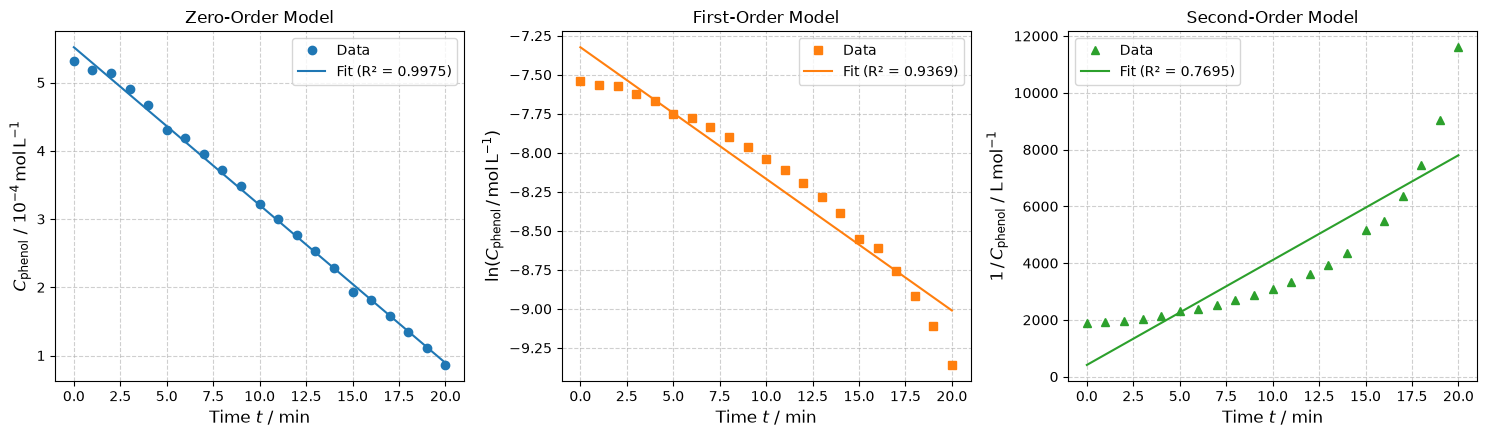
\includegraphics[width=\linewidth,keepaspectratio]{task1_phenol_reaction_order_fits.png}
  \caption{Linearized phenol concentration data for determining the reaction
  order in Task 1.}
  \label{fig:task1-order}
\end{figure}

\begin{table}[htbp]
  \centering
  \caption{Integral-method regression results for determining the reaction
  order with respect to phenol.}
  \label{tab:task1-phenol-order}
  \small
  \begin{tabular}{lrrrr}
    \toprule
    Reaction order & Linearized form & Slope & Intercept & \(R^2\) \\
    \midrule
    Zero order  & \(C(t)\)    & \(-0.000023\) & \(0.000552\) & \(0.997547\) \\
    First order & \(\ln C(t)\) & \(-0.084342\) & \(-7.323563\) & \(0.936867\) \\
    Second order & \(1/C(t)\) & \(369.304894\) & \(413.319621\) & \(0.769527\) \\
    \bottomrule
  \end{tabular}
\end{table}
The reported slope and intercept values follow the linearized variables
shown in Fig.~\ref{fig:task1-order}, using \(C\) in \si{mol/L} and time in
\si{min}.

\paragraph{Determination of the reaction order with respect to copper(II) sulfate}
The reaction order \(\gamma\) with respect to copper(II) sulfate was
determined at a constant temperature of \(T=\SI{70}{\degreeCelsius}\) and a
constant initial AP concentration of
\(C_{\mathrm{AP}}^{0}=\SI{5}{g/L}\) for all experimental runs. Equation
\eqref{eq:task1-kapp} can then be written as
\begin{equation}
  k_{\mathrm{app}} = K'\,(C_{\mathrm{CuSO_4}}^{0})^{\gamma},
  \qquad
  K' = k(\SI{70}{\degreeCelsius})\,(C_{\mathrm{AP}}^{0})^{\beta}.
  \label{eq:task1-catalyst-kapp}
\end{equation}
Taking logarithms gives the linear form
\begin{equation}
  \ln(k_{\mathrm{app}})
    = \ln(K') + \gamma\,\ln(C_{\mathrm{CuSO_4}}^{0}).
  \label{eq:task1-catalyst-linear}
\end{equation}
The values of \(k_{\mathrm{app}}\) were obtained from the slopes of the
regressions described above. The four experimental runs with different
copper(II) sulfate concentrations therefore provide four data points for the
regression in Eq.~\eqref{eq:task1-catalyst-linear}. The graphical and
analytical results are presented in Fig.~\ref{fig:task1-catalyst} and
Table~\ref{tab:task1-catalyst-results}. The estimated reaction order is
\(\gamma=0.33\).

\begin{figure}[htbp]
  \centering
  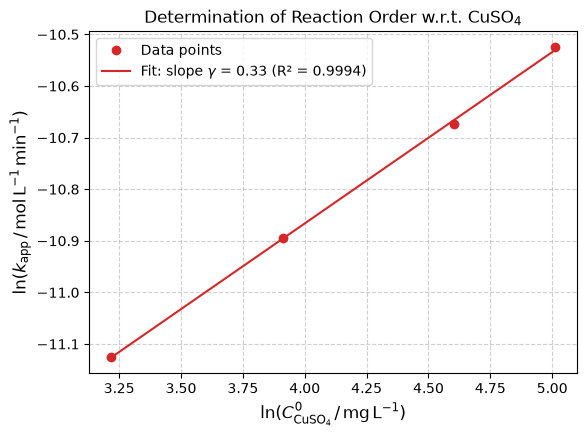
\includegraphics[width=0.8\linewidth,keepaspectratio]{task1_cuso4_reaction_order_fit.png}
  \caption{Determination of the reaction order with respect to copper(II)
  sulfate.}
  \label{fig:task1-catalyst}
\end{figure}

\begin{table}[htbp]
  \centering
  \caption{Apparent rate constants obtained at different initial copper(II)
  sulfate concentrations at \SI{70}{\degreeCelsius}.}
  \label{tab:task1-catalyst-results}
  \small
  \setlength{\tabcolsep}{4pt}
  \begin{tabular}{rrrrr}
    \toprule
    \(C_{\mathrm{CuSO_4}}^0\) (\si{mg/L}) &
    \(\ln C_{\mathrm{CuSO_4}}^0\) &
    \(k_{\mathrm{app}}\) (\si{mol/(L.min)}) &
    \(\ln k_{\mathrm{app}}\) &
    \(R^2\) \\
    \midrule
    25  & 3.218876 & 0.000015 & -11.124366 & 0.996130 \\
    50  & 3.912023 & 0.000019 & -10.894630 & 0.997372 \\
    100 & 4.605170 & 0.000023 & -10.674290 & 0.997547 \\
    150 & 5.010635 & 0.000027 & -10.524115 & 0.997567 \\
    \bottomrule
  \end{tabular}
\end{table}

The regression of \(\ln(k_{\mathrm{app}})\) against
\(\ln(C_{\mathrm{CuSO_4}}^0)\) gave
\(\gamma=0.332\) with \(R^2=0.9994\).

\paragraph{Determination of the activation energy}
The activation energy was determined using the logarithmic form of the
Arrhenius equation:
\begin{equation}
  \ln(k_{\mathrm{app}}(T))
    = \ln(A_{\mathrm{app}})
      - \frac{E_{\mathrm{A}}}{R}\,\frac{1}{T}.
  \label{eq:task1-arrhenius}
\end{equation}
For each temperature, a linear regression was performed on the corresponding
experimental time series, as in the preceding analyses, to determine
\(k_{\mathrm{app}}\). The relevant measurements are provided in
Table~\ref{tab:task1-temperature-data}. The zero-order fits for the
temperature-dependent runs are shown in Fig.~\ref{fig:task1-temperature-fits}.
The Arrhenius plot and regression results are presented in
Fig.~\ref{fig:task1-arrhenius} and Table~\ref{tab:task1-arrhenius-results}. For the Arrhenius plot,
\(\ln(k_{\mathrm{app}})\) is plotted against \(1/T\), with the temperature
expressed in kelvin. The slope \(m\) of the regression line is
\(-E_{\mathrm{A}}/R\), and hence
\begin{equation}
  E_{\mathrm{A}} = -mR,
  \label{eq:task1-activation-energy}
\end{equation}
where \(E_{\mathrm{A}}\) is obtained in \si{J/mol} when \(R\) is expressed in
\si{J/(mol.K)}; it may then be converted to \si{kJ/mol}.

\begin{table}[htbp]
  \centering
  \caption{Apparent rate constants and individual regression results for the
  temperature-dependent runs.}
  \label{tab:task1-temperature-data}
  \small
  \setlength{\tabcolsep}{4pt}
  \begin{tabular}{rrrrrr}
    \toprule
    \(T\) (\si{\degreeCelsius}) &
    \(T\) (\si{K}) &
    \(1/T\) (\si{K^{-1}}) &
    \(k_{\mathrm{app}}\) (\si{mol/(L.min)}) &
    \(\ln k_{\mathrm{app}}\) &
    \(R^2\) \\
    \midrule
    60 & 333.15 & 0.003002 & 0.000009 & -11.657132 & 0.998387 \\
    65 & 338.15 & 0.002957 & 0.000014 & -11.146147 & 0.998481 \\
    70 & 343.15 & 0.002914 & 0.000023 & -10.674290 & 0.997547 \\
    80 & 353.15 & 0.002832 & 0.000050 &  -9.900976 & 0.993688 \\
    \bottomrule
  \end{tabular}
\end{table}

\begin{figure}[htbp]
  \centering
  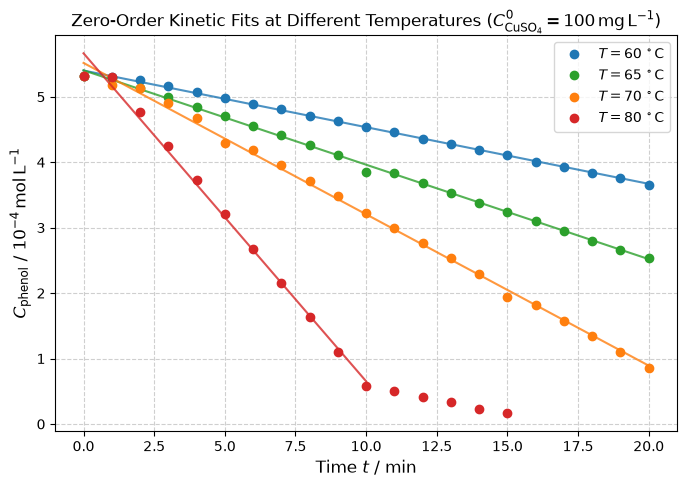
\includegraphics[width=\linewidth,keepaspectratio]{task1_zero_order_fits_temperatures.png}
  \caption{Zero-order fits to the phenol concentration profiles at different
  temperatures in Task 1.}
  \label{fig:task1-temperature-fits}
\end{figure}

\begin{figure}[htbp]
  \centering
  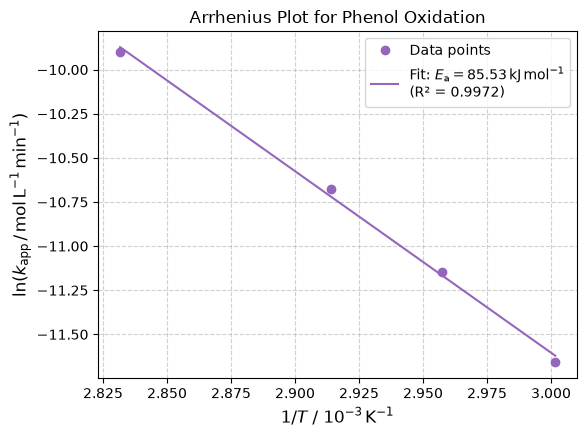
\includegraphics[width=0.8\linewidth,keepaspectratio]{task1_arrhenius_plot_phenol.png}
  \caption{Arrhenius plot for determining the activation energy in Task 1.}
  \label{fig:task1-arrhenius}
\end{figure}

\begin{table}[htbp]
  \centering
  \caption{Regression results for the Arrhenius analysis.}
  \label{tab:task1-arrhenius-results}
  \begin{tabular}{ll}
    \toprule
    Result & Value \\
    \midrule
    Regression slope, \(m=-E_{\mathrm{A}}/R\) & \(-10287.57\ \si{K}\) \\
    Intercept, \(\ln(A_{\mathrm{app}})\) & \(19.2587\) \\
    Activation energy, \(E_{\mathrm{A}}\) & \(\SI{85.53}{kJ/mol}\) \\
    Pre-exponential factor, \(A_{\mathrm{app}}\) & \(\SI{2.312e8}{mol/(L.min)}\) \\
    Regression coefficient, \(R^2\) & \(0.9972\) \\
    \bottomrule
  \end{tabular}
\end{table}

\subsection{Task 2}

The reaction order and rate constant were first determined by linearizing the
concentration profiles according to the integral method for zero-, first-, and
second-order reactions, as in Task 1. The reaction order and rate constant
were obtained from the best-fitting linearization. The results are
reported in Table~\ref{tab:task2-integral-results}. The linearized fits are shown in
Fig.~\ref{fig:task2-order}.

\begin{figure}[htbp]
  \centering
  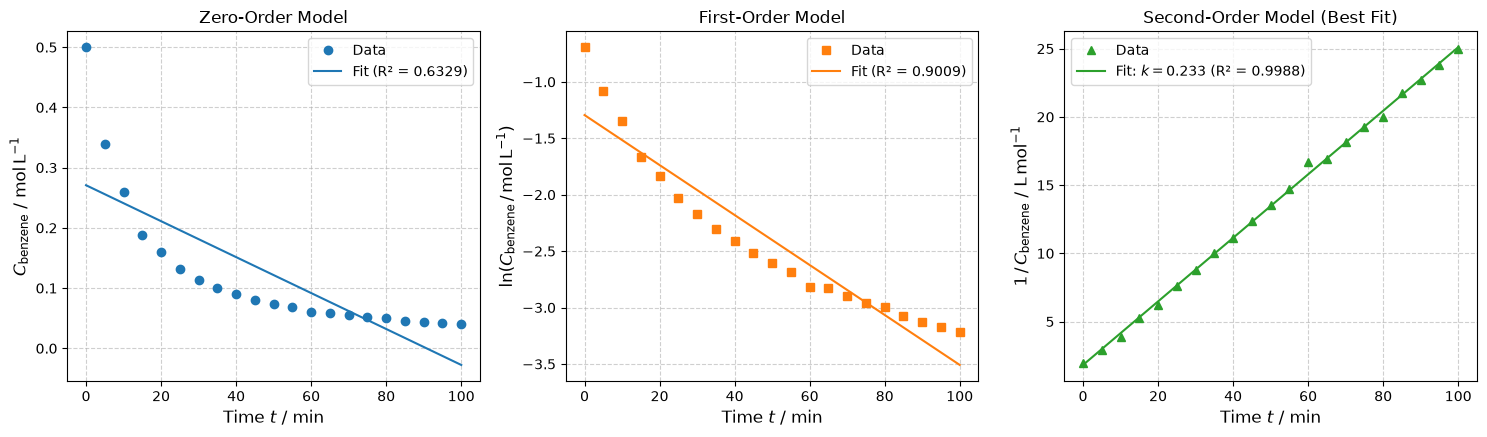
\includegraphics[width=\linewidth,keepaspectratio]{task2_benzene_reaction_order_fits.png}
  \caption{Integral-method fits for determining the reaction order of benzene
  decomposition in Task 2.}
  \label{fig:task2-order}
\end{figure}

\begin{table}[htbp]
  \centering
  \caption{Integral-method regression results for benzene decomposition at
  \SI{30}{\degreeCelsius}.}
  \label{tab:task2-integral-results}
  \small
  \setlength{\tabcolsep}{4pt}
  \begin{tabular}{lcrrrr}
    \toprule
    Reaction order & Linearized form & Slope & Intercept & \(R^2\) &
    \(k\) \\
    \midrule
    Zero order & \(C(t)\) & \(-0.002984\) & \(0.270827\) & \(0.632865\) &
    \(\SI{0.002984}{mol/(L.min)}\) \\
    First order & \(\ln C(t)\) & \(-0.022140\) & \(-1.294354\) & \(0.900894\) &
    \(\SI{0.022140}{min^{-1}}\) \\
    Second order & \(1/C(t)\) & \(0.232823\) & \(1.821871\) & \(0.998840\) &
    \(\SI{0.232823}{L/(mol.min)}\) \\
    \bottomrule
  \end{tabular}
\end{table}

The second-order model gave the highest \(R^2\); accordingly, the selected
reaction order is \(n=2\), and \(k_1=\SI{0.232823}{L/(mol.min)}\).

\begin{table}[htbp]
  \centering
  \caption{Summary of the Arrhenius extrapolation and half-life calculation
  for Task 2.}
  \label{tab:task2-extrapolation}
  \begin{tabular}{ll}
    \toprule
    Parameter & Value \\
    \midrule
    \(k_1\) at \(\SI{30}{\degreeCelsius}\) &
      \(\SI{0.2328}{L/(mol.min)}\) \\
    \(E_{\mathrm{A}}/R\) & \(\SI{13386.4}{K}\) \\
    \(1/T_1-1/T_2\) & \(\SI{2.0416e-4}{K^{-1}}\) \\
    \(k_2/k_1\) & \(15.38\) \\
    \(k_2\) at \(\SI{50}{\degreeCelsius}\) &
      \(\SI{3.580}{L/(mol.min)}\) \\
    \(k_2\) at \(\SI{50}{\degreeCelsius}\), converted &
      \(\SI{0.0597}{L/(mol.s)}\) \\
    Initial concentration, \(C_0\) & \(\SI{1.282}{mol/L}\) \\
    Half-life at \(\SI{50}{\degreeCelsius}\) &
      \(\SI{0.22}{min}\) (\(\SI{13.1}{s}\)) \\
    \bottomrule
  \end{tabular}
\end{table}

Next, the rate constant at \(\SI{50}{\degreeCelsius}\) was determined using the 
integrated Arrhenius equation: \begin{equation} \ln\!\left(\frac{k_2}{k_1}\right) = \frac{E_{\mathrm{A}}}{R} \left(\frac{1}{T_1}-\frac{1}{T_2}\right). \label{eq:task2-integrated-arrhenius} \end{equation} 
Using the parameters summarized in Table~\ref{tab:task2-extrapolation}, the rate constant 
at \(\SI{50}{\degreeCelsius}\) was calculated as \begin{equation} k_2 \approx \SI{3.580}{L/(mol.min)} \approx \SI{0.0597}{L/(mol.s)}. \label{eq:task2-k-at-50} \end{equation} 
For a second-order reaction, the half-life is given by \begin{equation} t_{1/2} = \frac{1}{k_2 C_0}. \label{eq:task2-half-life} \end{equation} 
The initial concentration was obtained from the ratio of mass concentration and molar mass, yielding \(C_0 = \SI{1.282}{mol/L}\). 
Substituting \(C_0\) and the calculated rate constant into Eq.~\eqref{eq:task2-half-life} gives \begin{equation} t_{1/2} \approx \SI{0.22}{min} \approx \SI{13.1}{s}. \label{eq:task2-half-life-result} \end{equation}

\subsection{Task 3}

The kinetic parameters for this system were determined using the differential
method of van't Hoff. Because only a small number of data points were
available, a polynomial was first fitted to the measurements. This
approximation was used to represent the concentration profile over the
experimental time interval. Reaction rates were then estimated from the
smoothed profile using centered finite differences:
\begin{equation}
  r(t_i) \approx -\frac{\Delta C}{\Delta t}
    = \frac{C_{i-1}-C_{i+1}}{t_{i+1}-t_{i-1}}.
  \label{eq:task3-rate-estimate}
\end{equation}
Polynomial fits of degrees 1 through 5 were compared using \(R^2\), as
summarized in Table~\ref{tab:task3-polynomial-fits}. The degree-5 polynomial
was used to smooth the concentration profile. The derived differential rates
and corresponding concentrations are listed in
Table~\ref{tab:task3-differential-data}.

\begin{table}[htbp]
  \centering
  \caption{Polynomial fits compared for smoothing the Task 3 concentration
  profile.}
  \label{tab:task3-polynomial-fits}
  \scriptsize
  \setlength{\tabcolsep}{3pt}
  \begin{tabular}{rrp{0.78\linewidth}}
    \toprule
    Degree & \(R^2\) & Fitted concentration polynomial, \(C(t)\) \\
    \midrule
    1 & 0.89046 &
      \(\begin{aligned}
        C(t) &= -1.4487\times10^{-2}t + 0.8329
      \end{aligned}\) \\
    2 & 0.99297 &
      \(\begin{aligned}
        C(t) &= 3.1120\times10^{-4}t^2 - 3.2775\times10^{-2}t\\
             &\quad + 0.9572
      \end{aligned}\) \\
    3 & 0.99905 &
      \(\begin{aligned}
        C(t) &= -5.1973\times10^{-6}t^3 + 7.8125\times10^{-4}t^2\\
             &\quad - 4.3229\times10^{-2}t + 0.9887
      \end{aligned}\) \\
    4 & 0.99984 &
      \(\begin{aligned}
        C(t) &= 1.0437\times10^{-7}t^4 - 1.7600\times10^{-5}t^3\\
             &\quad + 1.2370\times10^{-3}t^2 - 4.8518\times10^{-2}t\\
             &\quad + 0.9978
      \end{aligned}\) \\
    5 & 1.00000 &
      \(\begin{aligned}
        C(t) &= -4.2846\times10^{-9}t^5 + 7.3638\times10^{-7}t^4\\
             &\quad - 4.9537\times10^{-5}t^3 + 1.8665\times10^{-3}t^2\\
             &\quad - 5.2357\times10^{-2}t + 1.0002
      \end{aligned}\) \\
    \bottomrule
  \end{tabular}
\end{table}

\begin{table}[htbp]
  \centering
  \caption{Concentrations and differential reaction rates used in Task 3.}
  \label{tab:task3-differential-data}
  \scriptsize
  \setlength{\tabcolsep}{4pt}
  \begin{tabular}{rrrrrr}
    \toprule
    \(t\) (\si{s}) &
    \(c_{\mathrm{real}}\) (\si{mol/L}) &
    \(c_{\mathrm{poly}}\) (\si{mol/L}) &
    \(r\) (\si{mol/(L.s)}) &
    \(\ln(c)\) &
    \(\ln(r)\) \\
    \midrule
     0.0 & 1.0000 & 1.0002 & \(5.23568\times10^{-2}\) &  0.0002 & -2.9497 \\
     5.0 & 0.7800 & 0.7793 & \(3.70525\times10^{-2}\) & -0.2493 & -3.2954 \\
    10.0 & 0.6200 & 0.6207 & \(2.71570\times10^{-2}\) & -0.4770 & -3.6061 \\
    25.0 & 0.3300 & 0.3296 & \(1.42585\times10^{-2}\) & -1.1098 & -4.2504 \\
    35.0 & 0.2100 & 0.2103 & \(9.60861\times10^{-3}\) & -1.5594 & -4.6451 \\
    50.0 & 0.1200 & 0.1199 & \(2.93568\times10^{-3}\) & -2.1209 & -5.8308 \\
    60.0 & 0.0900 & 0.0900 & \(4.78149\times10^{-3}\) & -2.4078 & -5.3430 \\
    \bottomrule
  \end{tabular}
\end{table}

The differential rate law and its linearized form are
\begin{equation}
  r = kC^n,
  \qquad
  \ln(r) = \ln(k) + n\ln(C).
  \label{eq:task3-linearized-rate-law}
\end{equation}
The data are plotted in the linearized form shown in
Eq.~\eqref{eq:task3-linearized-rate-law}; the plot is included as
Fig.~\ref{fig:task3-differential-plot}. The plot is discontinuous at its
left-hand end, so the analysis was restricted to the linear region. This
region was selected iteratively by filtering the data, as documented in the
Python code. The slope of the regression over the selected region gives the
reaction order \(n\), while the intercept gives \(\ln(k)\), from which \(k\)
is obtained by exponentiation. The results are reported in
Table~\ref{tab:task3-kinetic-results}.

\begin{figure}[htbp]
  \centering
  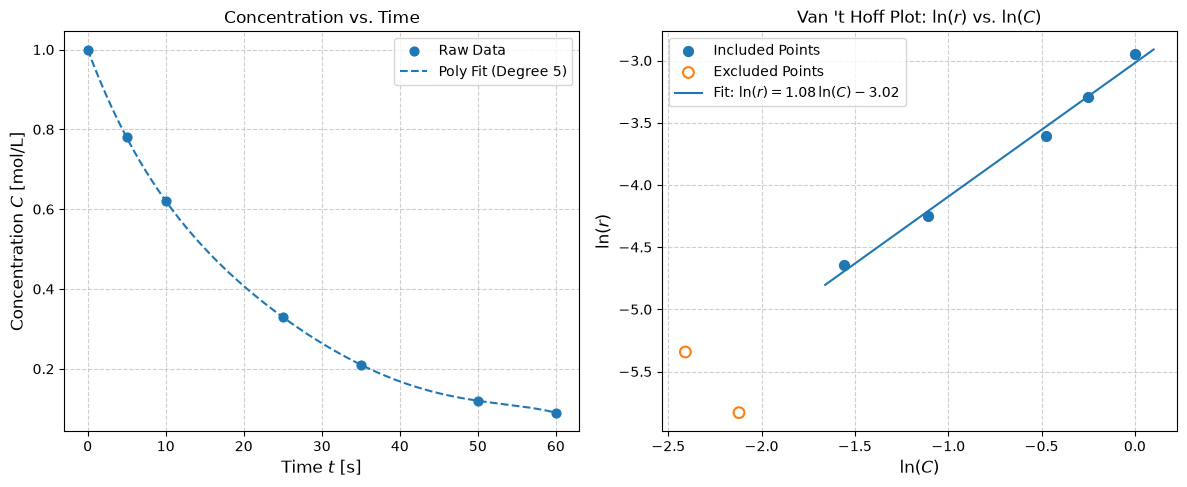
\includegraphics[width=\linewidth,keepaspectratio]{task3_van_t_hoff_differential_method.png}
  \caption{Concentration profile and linearized differential-rate data with
  the fitted region for Task 3.}
  \label{fig:task3-differential-plot}
\end{figure}

\begin{table}[htbp]
  \centering
  \caption{Kinetic results obtained from the differential analysis in Task 3.}
  \label{tab:task3-kinetic-results}
  \begin{tabular}{ll}
    \toprule
    Result & Value \\
    \midrule
    Overall reaction order, \(n\) & \(1.0753\) \\
    Rate constant, \(k\) & \(4.8844\times10^{-2}\,
      (\si{L/mol})^{0.08}\si{s^{-1}}\) \\
    Fit quality, \(R^2\) & \(0.99251\) \\
    Points included in final regression & \(0\) to \(4\) \\
    \bottomrule
  \end{tabular}
\end{table}

The value of \(n\) represents the overall reaction order, not the partial
order with respect to N-acetylcysteine. Determining the partial order would
require separate experiments in which the other component concentrations
were held in excess. Such experiments were not performed here because the
reactants were present as an equimolar mixture.
